\section{Project planning}
\subsection{Tentative time-plan}
	\begin{tabular}{ll}
	10. Feb & Delivery of preliminary report\\
	 & Schedule for time-period between 27.01.2013 and 10.02.2013\\
	15. Mar & Delivery of mid term report\\
	  & Schedule for time-perood between 10.02.2013 and 15.03.2013\\
	27. May & Delivery of final report\\
	 & Schedule for time-period between 15.03.2013 and 27.05.2013\\  
\end{tabular}
\begin{figure}[H]
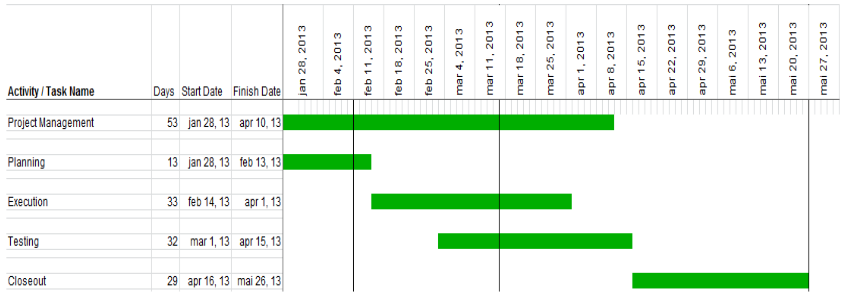
\includegraphics[scale=0.8]{images/gantt-diagram.png}
\caption{Gantt diagram. Milestones are marked using vertical lines}
\end{figure}
\subsection{Development method}
Iterative model based on lean with proposal to the customer weekly. This agile methodology decreased the project risk and secured a complete and functional system for the customer. The customer could then influence our work and adjust potential misconceptions early in the project. Prototypes and demonstration for SINTEF was made in the beginning to validate our understanding of the requirements.\\
\newline
Our team was grouped into three, which made it easy to do pair-programming and individual work.
\subsection{Risk analysis}
\captionof{table}{Risk analysis}
\label{fig:risktable}
\begin{longtable}{|m{0.15 \textwidth}|m{0.1 \textwidth}|m{0.1 \textwidth}|m{0.1 \textwidth}|m{0.185 \textwidth}|m{0.185 \textwidth}|}
\hline
	\rowcolor{Gray}
	\textbf{Description} & \textbf{Likeli{-}hood} & \textbf{Impact} & \textbf{Impor{-}tance} & \textbf{Preventive\newline Action} & \textbf{Remedial\newline Action}\\
	\endfirsthead%
	\multicolumn{6}{l}%
	{{\bfseries Continued from previous page}} \\ \hline
	\rowcolor{Gray}
	\textbf{Description} & \textbf{Likeli{-}hood} & \textbf{Impact} & \textbf{Impor{-}tance} & \textbf{Preventive\newline Action} & \textbf{Remedial\newline Action}\\
\hline
	\endhead%
	\hline

	\hline \multicolumn{6}{|l|}{{Continued on next page}} \\ \hline
	\endfoot%

	\endlastfoot%

	Illness & 7 & 2 & 14 & Good\newline communication and effective use of GitHub & Increase workhours and exchange tasks and\newline responsibilities\\
\hline
	Project\newline complexity & 6 & 5 & 30 & Don't take on too much work & Cut down the demands\\
\hline
	Customer\newline issues & 1 & 5 & 5 & Agreement with customer and weekly feedback from customer & Use the\newline original\newline requirement specification\\
\hline
	License\newline incompability & 7 & 7 & 49 & Avoid\newline integrating components with incopatible licenses & Discover other implementations or implment from scratch\\
\hline
	Group\newline conflicts or disagreements & 3 & 3 & 9 & Keep close\newline contact to avoid\newline surprises.\newline Leader takes\newline action & Contact\newline supervisor and make an\newline appointment\\
\hline
	Over the air complexity & 8 & 8 & 64 & Have multiple\newline alternative\newline solutions and keep close\newline contact with customer & Detail what was attempted as well as why it couldn't be solved in the final report.\\
\hline
	Personal matters & 8 & 5 & 40 & Not much\newline preventative action can be taken & Keep in touch and stay\newline updated. In case you still can do tasks, claim one and tell the\newline others\\
\hline
\end{longtable}
\subsection{Architectural scetch}
The market application is made for Android platform 2.2 or 2.3 and above. This depends on the the difficulties in creation of the application. It consist of a list of available apps for Arduinos and a requirement section to see what equipment and hardware that is required for each app.
